\documentclass{ximera}

\title{Theory}
\author{Mila Vervoort}
\license{CC: 0}         % replace with an appropriate license, or set it in xmPreamble

\begin{document}
\begin{abstract}
    Samenvatting van de theorie over ideale homogene reactoren onder isotherme voorwaarden.
\end{abstract}
\maketitle
\label{xim:theory}

In hoofdstuk 3 'Ontwerp van homogene reaktoren onder isotherme werkingsvoorwaarden' werd gezien hoe door het opstellen van de stofbalans de nodige ontwerpvergelijkingen bekomen kunnen worden. 

Een stofbalans is van de volgende vorm: 
\[
\text{Accumulation} = \text{In} - \text{Uit} + \text{Vorming} - \text{Verbruik}
\]
In formulevorm:
\[
\frac{dN_A}{dt} = F_{A,in} - F_{A,out} + R_A V
\]
waar:
\begin{itemize}
\item $N_A$ = aantal mol van component A in de reactor
\item $F_{A,in}$ = molstroom van A naar binnen
\item $F_{A,out}$ = molstroom van A naar buiten
\item $R_A$ = reactiesnelheid van A (mol/(m$^3$s))
\item $V$ = reactorvolume
\end{itemize}

\begin{remark}
Monotoon stijgende kinetica

We veronderstellen een monotoom stijgende kinetiek in het vervolg van de theorie.
Voor een irreversibele reactie met monotoon stijgende kinetica geldt:

\[
R_A = \frac{dC_A}{dt} = -k C_A^n
\]

waarbij:

\begin{itemize}
\item $n=1$ : eerste orde
\item $n=2$ : tweede orde
\item $n=3$ : derde orde
\item $\dots$
\end{itemize}

Hieruit volgt:

\[
-\frac{1}{R_A} = \frac{1}{k C_A^n}
\]

De onderstaande grafiek toont $-1/R_A$ als functie van $C_A$
voor verschillende waarden van $n$. 

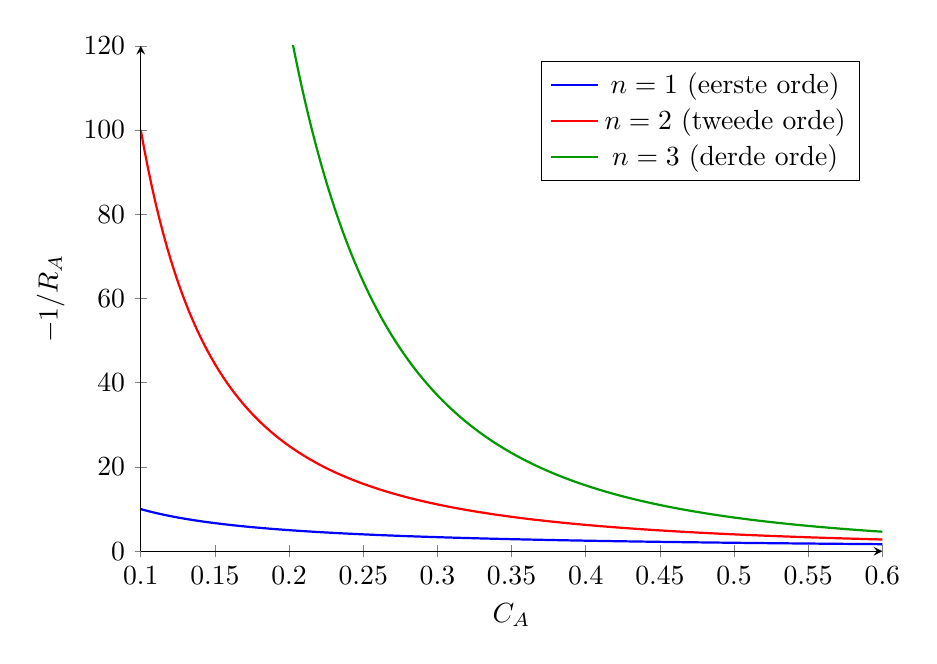
\begin{tikzpicture}
\begin{axis}[
    xlabel={$C_A$},
    ylabel={$-1/R_A$},
    domain=0.1:0.6,
    samples=200,
    axis lines=left,
    width=11cm,
    height=8cm,
    legend pos=north east,
    ymin=0,
    ymax=120,
]

% n = 1
\addplot[blue, thick] {1/x};
\addlegendentry{$n=1$ (eerste orde)}

% n = 2
\addplot[red, thick] {1/(x^2)};
\addlegendentry{$n=2$ (tweede orde)}

% n = 3
\addplot[green!60!black, thick] {1/(x^3)};
\addlegendentry{$n=3$ (derde orde)}

\end{axis}
\end{tikzpicture}
\end{remark}


 
\section{Batch Reactor}

In een batch reactor is er geen in- of uitstroom (\(F_{A,in} = F_{A,out} = 0\)):

\[
\frac{dN_A}{dt} = R_A V
\]

Aangezien $N_A = N_{A0}(1-X_A)$:

\[
\frac{dX_A}{dt} = \frac{-r_A}{C_{A0}}
\]

Om de tijd \(t\) te berekenen die nodig is om van een initiële conversie \(X_{A0} = 0\) naar conversie \(X_A\) te gaan, integreren we:

\[
\boxed{
t = \int_0^{X_A} \frac{C_{A0}}{-r_A}\, dX_A
}
\]

\begin{image}
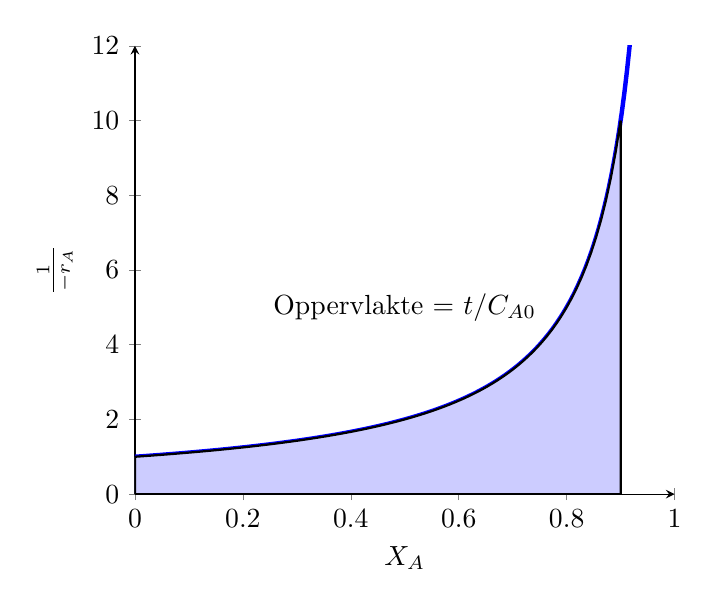
\begin{tikzpicture}
\begin{axis}[
    domain=0:0.95,
    samples=200,
    xmin=0, xmax=1,
    ymin=0, ymax=12,
    axis lines=left,
    xlabel={$X_A$},
    ylabel={$\frac{1}{-r_A}$},
]

% parameters
\addplot[ultra thick, blue]
{1/(1*(1-x))};

% arceer het gebied tussen C_A_end en C_A0
\addplot [
    thick,
    fill=blue!20,
    domain=0:0.9,   % van C_A,e tot C_A0
    samples=100
] {1/(1*(1-x))} \closedcycle;

% Voeg een t label toe in het gearceerde gebied
\node at (axis cs:0.5,5) {Oppervlakte = $t/C_{A0}$};

\end{axis}
\end{tikzpicture}
\end{image} 

Bij de aanname van constante densiteit:

\[
\frac{dC_A}{dt} = r_A
\]

Om de tijd \(t\) te berekenen die nodig is om van een initiële concentratie \(C_{A0}\) naar \(C_A\) te gaan, integreren we:
\[
\boxed{
t = \int_{C_{A0}}^{C_A} \frac{dC_A}{r_A}
}
\]

\begin{image}
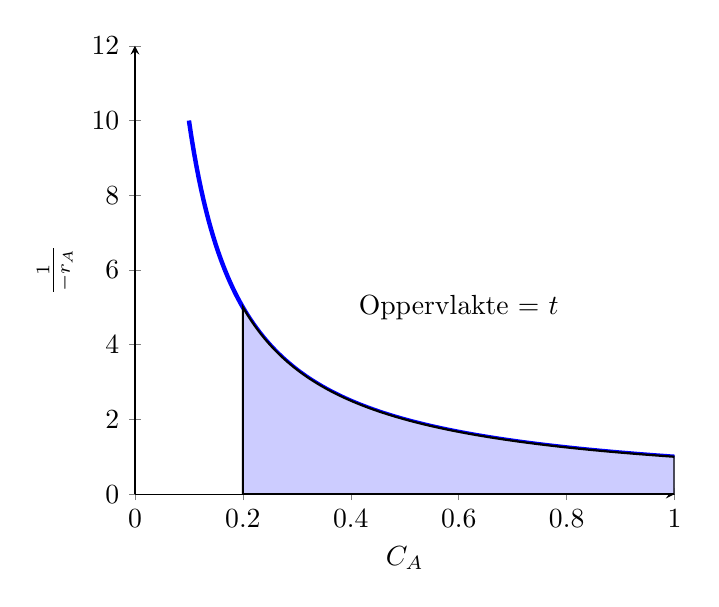
\begin{tikzpicture}
\begin{axis}[
    domain=0.1:1,       % x loopt van 0 tot C_A0
    samples=200,
    xmin=0, xmax=1,
    ymin=0, ymax=12,
    axis lines=left,
    xlabel={$C_A$},
    ylabel={$\frac{1}{-r_A}$},
]

% parameters
\def\k{1}   % snelheidsconstante

% plot de curve
\addplot[ultra thick, blue] {1/(\k*x)};

% arceer het gebied tussen C_A_end en C_A0
\addplot [
    thick,
    fill=blue!20,
    domain=0.2:1,   % van C_A,e tot C_A0
    samples=100
] {1/(\k*x)} \closedcycle;

% Voeg een t label toe in het gearceerde gebied
\node at (axis cs:0.6,5) {Oppervlakte = $t$};

\end{axis}
\end{tikzpicture}
\end{image}


\section{CSTR (Continuous Stirred Tank Reactor)}

In een CSTR met constante in- en uitstroom geldt bij stationaire toestand:

\[
0 = F_{A0}-F_A+r_A V
\]

\[
F_{A0}X_A = -r_A V
\]

\[
\boxed{
\frac{V}{F_{A0}} = \frac{dX_{A,e}}{-r_A}
}
\]

\begin{image}
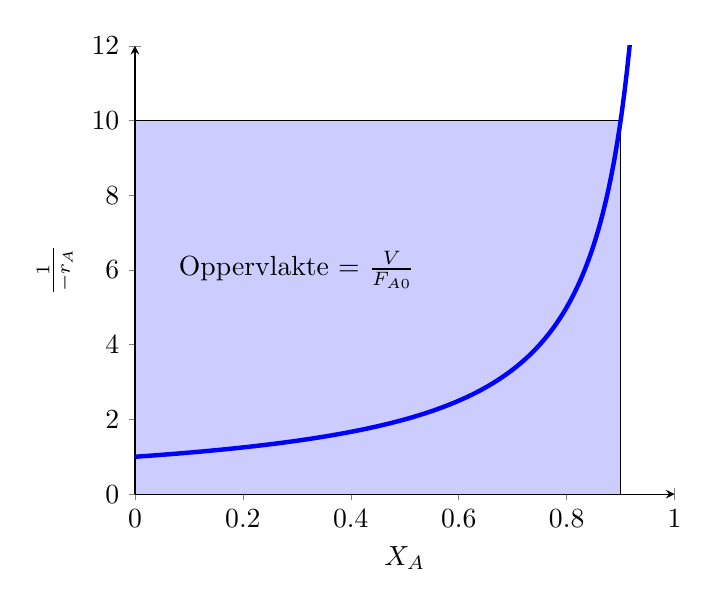
\begin{tikzpicture}
\begin{axis}[
    domain=0:0.95,
    samples=200,
    xmin=0, xmax=1,
    ymin=0, ymax=12,
    axis lines=left,
    xlabel={$X_A$},
    ylabel={$\frac{1}{-r_A}$},
]


% arceer het gebied 
\draw[fill=blue!20] 
    (axis cs:0,0) rectangle 
    (axis cs:0.9,{1/(1-0.9)});

% parameters
\addplot[ultra thick, blue]
{1/(1*(1-x))};

\node at (axis cs:0.3,6) {Oppervlakte = $\frac{V}{F_{A0}}$};


\end{axis}
\end{tikzpicture}
\end{image} 

Bij de aanname van constante densiteit:

\[
\boxed{
\tau = \frac{C_{A0}-C_{Ae}}{-r_A}
}
\]


\begin{image}
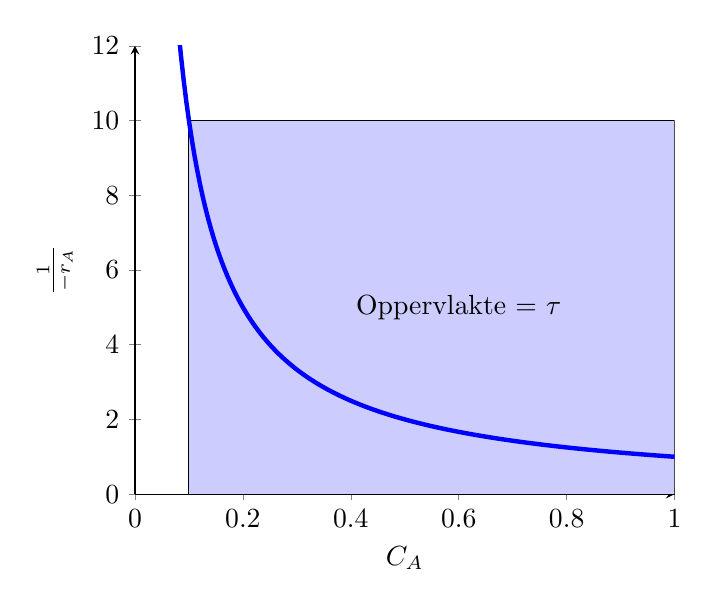
\begin{tikzpicture}
\begin{axis}[
    domain=0:1,       % x loopt van 0 tot C_A0
    samples=200,
    xmin=0, xmax=1,
    ymin=0, ymax=12,
    axis lines=left,
    xlabel={$C_A$},
    ylabel={$\frac{1}{-r_A}$},
]

% parameters
\def\k{1}   % snelheidsconstante



% arceer het gebied 

\draw[fill=blue!20] 
    (axis cs:1,0) rectangle 
    (axis cs:0.1,{1/0.1});
% plot de curve
\addplot[ultra thick, blue] {1/(\k*x)};
    
% Voeg een t label toe in het gearceerde gebied
\node at (axis cs:0.6,5) {Oppervlakte = $\tau$};

\end{axis}
\end{tikzpicture}
\end{image}


\section{PFR (Plug Flow Reactor)}

In een PFR verandert de concentratie langs de reactorlengte \(x\). De stofbalans over een klein segment \(dV\) is:


\[
\frac{dF_A}{dV} = r_A
\]

\[
\frac{dX_A}{dV} = \frac{-r_A}{F_{A0}}
\]

\[
\boxed{
\frac{V}{F_{A0}} = \int_0^{X_A}\frac{dX_A}{-r_A}
}
\]


\begin{image}
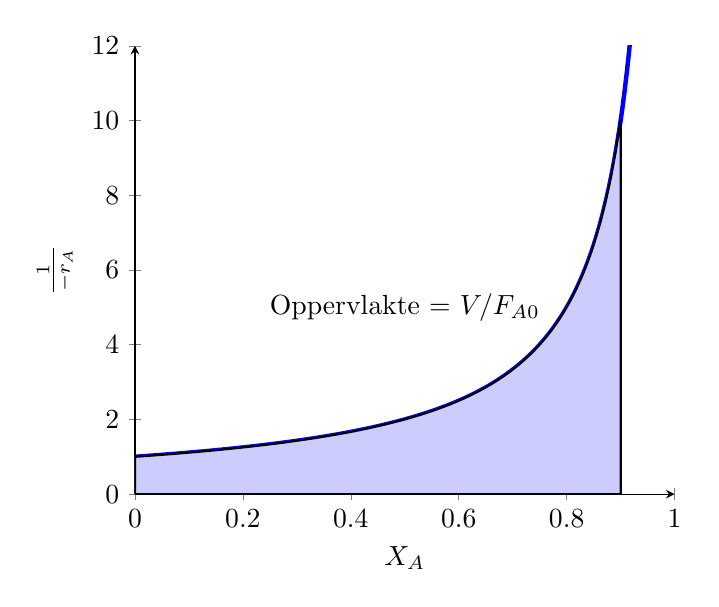
\begin{tikzpicture}
\begin{axis}[
    domain=0:0.95,
    samples=200,
    xmin=0, xmax=1,
    ymin=0, ymax=12,
    axis lines=left,
    xlabel={$X_A$},
    ylabel={$\frac{1}{-r_A}$},
]

% parameters
\addplot[ultra thick, blue]
{1/(1*(1-x))};

% arceer het gebied tussen C_A_end en C_A0
\addplot [
    thick,
    fill=blue!20,
    domain=0:0.9,   % van C_A,e tot C_A0
    samples=100
] {1/(1*(1-x))} \closedcycle;

% Voeg een t label toe in het gearceerde gebied
\node at (axis cs:0.5,5) {Oppervlakte = $V/F_{A0}$};

\end{axis}
\end{tikzpicture}
\end{image} 

Bij de aanname van constante densiteit:

\[
\boxed{
\tau = \int_0^{X_A}\frac{C_{A0}}{-r_A} dX_A
}
\]

\begin{image}
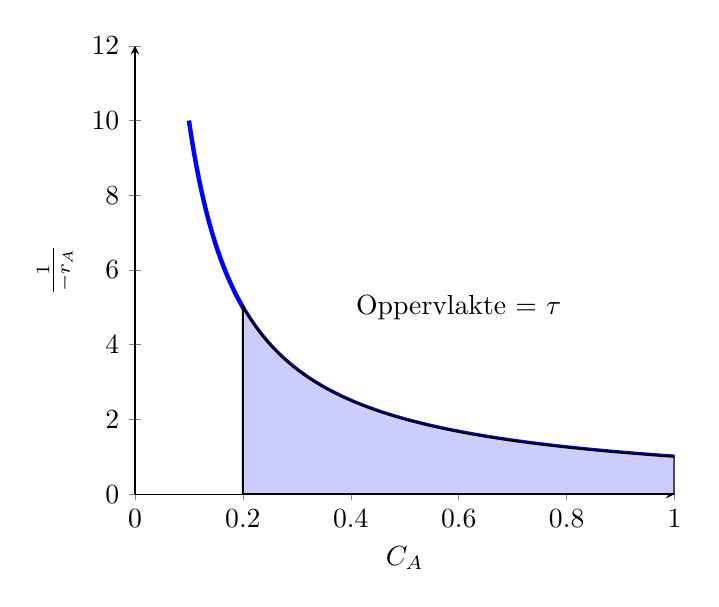
\begin{tikzpicture}
\begin{axis}[
    domain=0.1:1,       % x loopt van 0 tot C_A0
    samples=200,
    xmin=0, xmax=1,
    ymin=0, ymax=12,
    axis lines=left,
    xlabel={$C_A$},
    ylabel={$\frac{1}{-r_A}$},
]

% parameters
\def\k{1}   % snelheidsconstante

% plot de curve
\addplot[ultra thick, blue] {1/(\k*x)};

% arceer het gebied tussen C_A_end en C_A0
\addplot [
    thick,
    fill=blue!20,
    domain=0.2:1,   % van C_A,e tot C_A0
    samples=100
] {1/(\k*x)} \closedcycle;

% Voeg een t label toe in het gearceerde gebied
\node at (axis cs:0.6,5) {Oppervlakte = $\tau$};

\end{axis}
\end{tikzpicture}
\end{image}

\section{Vergelijking van ideale reactoren}
\subsection{Vergelijking: CSTR vs PFR}

We vergelijken de verblijftijd voor eenzelfde uitgangsconcentratie $C_A$.

\[
\tau_{PFR} = \int_{C_{A0}}^{C_A} \frac{dC_A}{r_A}
\]

\[
\tau_{CSTR} = \frac{C_{A0}-C_A}{-r_A|_{\text{uit}}}
\]

Grafisch in een $-1/r_A$ versus $C_A$ diagram:

\begin{center}
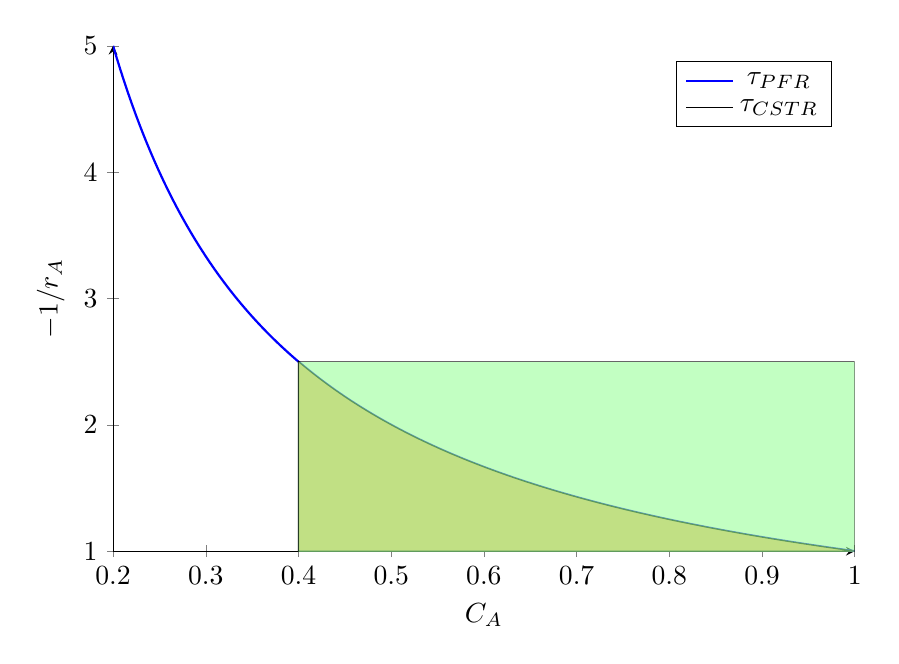
\begin{tikzpicture}
\begin{axis}[
    xlabel={$C_A$},
    ylabel={$-1/r_A$},
    domain=0.2:1,
    samples=200,
    axis lines=left,
    width=11cm,
    height=8cm,
    legend pos=north east,
]

% kinetiek
\addplot[blue, thick] {1/x};

% PFR oppervlakte
\addplot[
    domain=0.4:1,
    fill=orange!60
] {1/x} \closedcycle;
\addlegendentry{$\tau_{PFR}$}

% CSTR rechthoek
\draw[fill=green!40, opacity=0.6]
    (axis cs:1,0)
    rectangle
    (axis cs:0.4,{1/0.4});
\addlegendentry{$\tau_{CSTR}$}

\end{axis}
\end{tikzpicture}
\end{center}

\textbf{Interpretatie:}

Bij monotoon stijgende kinetica stijgt $-1/r_A$ bij dalende $C_A$.
De rechthoek (CSTR) is daardoor groter dan de integraal (PFR):

\[
\tau_{CSTR} > \tau_{PFR}
\]

Een PFR is dus efficiënter dan een CSTR voor dezelfde conversie.

Dit kan je ook zelf even uittesten:
\begin{center}
\geogebra{m4v7cs3y}{700}{700}
\end{center}

\subsection*{Vergelijking: Batch vs PFR}

Voor constante densiteit hebben Batch en PFR dezelfde
integraalvorm.

\begin{center}
\begin{tikzpicture}
\begin{axis}[
    xlabel={$C_A$},
    ylabel={$-1/r_A$},
    domain=0.2:1,
    samples=200,
    axis lines=left,
    width=11cm,
    height=8cm,
    legend pos=north east,
]

% kinetiek
\addplot[blue, thick] {1/x};
\addlegendentry{$-1/r_A$}

% PFR oppervlakte
\addplot[
    domain=0.4:1,
    fill=orange!40
] {1/x} \closedcycle;
\addlegendentry{$\tau_{PFR}$}

% Batch oppervlakte (zelfde gebied, andere kleur rand)
\addplot[
    domain=0.4:1,
    draw=red,
    pattern=north east lines,
    pattern color=red
] {1/x} \closedcycle;
\addlegendentry{$t_{Batch}$}

\end{axis}
\end{tikzpicture}
\end{center}

\textbf{Interpretatie:}

Bij constante densiteit is:

\[
t_{Batch} = \tau_{PFR}
\]

Batch en PFR volgen exact dezelfde integraal.
Het verschil is enkel operationeel:

\begin{itemize}
\item Batch: tijd evolueert in één vat
\item PFR: concentratie evolueert langs de reactorlengte
\end{itemize}





\section*{Samenvatting}

\begin{tabular}{|l|c|c|}
    \hline
    \textbf{Reactor Type} & \textbf{Stofbalans} & \textbf{Kernidee}\\
    \hline
    Batch & $\frac{dC_A}{dt} = R_A$ & Geen in-/uitstroom, alleen reactie\\
    CSTR & $Q C_{A,in} - Q C_{A,out} + R_A V = 0$ & Goed gemengd, stationaire toestand\\
    PFR & $\frac{dC_A}{dx} = \frac{R_A}{Q}$ & Concentratie verandert langs de lengte, plug-flow\\
    \hline
\end{tabular}


\end{document}